\section{The energy of a random arrangement}
\label{sec:random_energy}

Let $S$ be a uniformly random arrangement: $z_c=b_{\pi(c)}$ with $\pi$ uniform and $b$ the centred values $k-\frac{N+1}2$, $1\le k\le N$.
For a test function $\varphi$ put $T_\varphi=\Cov(\varphi,Z)=\sum_ca_cz_c$ with $a_c=(\varphi_c-\bar\varphi)/N$, a linear permutation statistic (\Cref{sec:bg_perm}).
$\Var(\varphi)$ and $\Cov(\varphi,\psi)$ denote population variances and covariances over the $N$ cells, and $\sigma_n^2=(n^2+1)/12$ as in \eqref{eq:sigma}.

\subsection{Means}

\begin{proposition}[Means and covariance structure]
\label{prop:random_energy_moments}
For all test functions $\varphi,\psi$, $\E[T_\varphi]=0$ and $\E[T_\varphi T_\psi]=\sigma_n^2\Cov(\varphi,\psi)$.
Consequently
\begin{gather}
\E\,\Cov(X,Z)^2=\E\,\Cov(Y,Z)^2=\frac{n^4-1}{144},\qquad
\E\,\Cov(\mathbf 1_L,Z)^2=\frac{(n-1)(n^2+1)}{12\,n^2}\ \text{ for every line }L,
\label{eq:single_terms}\\
\E[\Elow]=\frac{(n-1)(n^2+1)(n^3+n^2+12)}{72\,n^2},\qquad
\E[\Efull]=\frac{n^4-1}{6\,n^2}.
\label{eq:mean_low}
\end{gather}
The covariance matrix of the vector of statistics in $\Elow$ (resp.\ $\Efull$) is $\sigma_n^2\Gamma$, with $\Gamma$ the Gram matrix of the centred test functions; its eigenvalues are
\begin{equation}
\Elow:\ \sigma_n^2\Bigl\{\tfrac{n^2-1}{12}\,(\times2),\ \tfrac{n-1}{n^2}\,(\times2)\Bigr\},
\qquad
\Efull:\ \sigma_n^2\Bigl\{\tfrac1n\,(\times\,2n-2),\ \tfrac{n-1}{n^2}\,(\times2),\ 0\,(\times2)\Bigr\}
\label{eq:weights}
\end{equation}
for odd $n$; for even $n$ the pair $\{\tfrac{n-1}{n^2},\tfrac{n-1}{n^2}\}$ is replaced by $\{\tfrac1n,\tfrac{n-2}{n^2}\}$.
\end{proposition}

\begin{proof}
$\sum_ca_c=0$ gives $\E T_\varphi=0$, and \eqref{eq:ww_identity} with $\sum_j b_j^2=N\Var(Z)$ gives $\E[T_\varphi T_\psi]=\frac1{N-1}\cdot\frac{\Cov(\varphi,\psi)}{N}\cdot N\Var(Z)=\sigma_n^2\Cov(\varphi,\psi)$.
The entries of $\Gamma$ follow from \Cref{lem:W_structure}: $\Var(\mathbf 1_L)=(n-1)/n^2$, two lines meeting in $\ell$ cells have covariance $\ell/N-1/n^2$, and $X$, $Y$ are uncorrelated with each other and with the diagonal indicators, since a diagonal meets every row and every column once.
The rows give the block $\frac1n(I-\frac1nJ)$, the columns likewise, and the means are the traces.
\end{proof}

Equivalently, a line sum is the sum of a sample of size $n$ drawn without replacement from $\{1,\dots,N\}$, so $\E\delta_L^2=n\Var(Z)\frac{N-n}{N-1}$.
The means of the two energies coincide if and only if $\frac{n^2-1}{6}=\frac{2(n-1)}{n}$, i.e.\ $n=3$, where both equal $40/27$.

\begin{corollary}[Null distribution of Loly's invariant]
\label{cor:loly_null}
For a uniformly random arrangement, $I(S)$ of \Cref{cor:loly} satisfies
\begin{equation}
\E[I(S)]=\frac{n^{2}(n^{4}-1)}{12},\qquad
\Var\bigl(I(S)\bigr)=N^{2}\sigma_n^{2}\,\Var(X^{2}+Y^{2})=\frac{n^{4}(n^{4}-1)(n^{2}-4)}{1080}.
\label{eq:loly_null}
\end{equation}
The mean equals Loly's value for every distribution of arrangements invariant under relabelling of the values; magic and semi-magic squares sit exactly at the mean, with no fluctuation.
\end{corollary}

\begin{proof}
By \eqref{eq:loly_identity}, $I(S)-\frac{n^2(n^4-1)}{12}=N\,T_{X^2+Y^2}$, so \Cref{prop:random_energy_moments} gives the mean and $\Var(I)=N^2\sigma_n^2\Var(X^2+Y^2)$.
$X$ and $Y$ are independent and uniform on $n$ equally spaced points, so $\Var(X^2+Y^2)=2(\E X^4-(\E X^2)^2)$ with $\E X^2=\frac{n^2-1}{12}$ and $\E X^4=\frac{(n^2-1)(3n^2-7)}{240}$, which gives $\frac{(n^2-1)(n^2-4)}{90}$.
\end{proof}

For $n=3$, $\Var(I)=30$ and $I$ takes $29$ values from $46$ to $74$; for $n=4$, $\Var(I)=2176/3$ and $\Pr(I=340)=13049/450450\approx0.029$ (\texttt{anc/verify\_numbers.py}).

\subsection{Variances}

Write a random energy as a quadratic form $E=\sum_kT_{\varphi_k}^2=z^{\mathsf T}Az$ with $A=\sum_ka_ka_k^{\mathsf T}$, where $a_k=(\varphi_k-\bar\varphi_k)/N$.
$A$ is symmetric with zero row sums.

\begin{theorem}[Variance of a quadratic form in a random arrangement]
\label{thm:var_identity}
Let $A$ be a symmetric $N\times N$ matrix with zero row sums, $N\ge4$, and let $z$ be a uniformly random permutation of the centred values $k-\frac{N+1}2$, $1\le k\le N$.  Then $\E[z^{\mathsf T}Az]=\frac{N(N+1)}{12}\tr A$ and
\begin{equation}
\Var(z^{\mathsf T}Az)=-\frac{N(N+1)(2N+3)}{360}\,(\tr A)^2+\frac{N(N^2-1)(5N+6)}{360}\,\tr(A^2)-\frac{N^2(N+1)^2}{120}\sum_aA_{aa}^2 .
\label{eq:var_identity}
\end{equation}
\end{theorem}

\begin{proof}[Proof (sketch; details in \Cref{sec:app_variance})]
Expand $\E[(z^{\mathsf T}Az)^2]=\sum_{a,b,c,d}A_{ab}A_{cd}\E[z_az_bz_cz_d]$ according to the equality pattern of $(a,b,c,d)$, a set partition of $\{1,2,3,4\}$, and apply M\"obius inversion on the partition lattice, so that each pattern contributes an unrestricted sum.
An unrestricted sum in which some index occurs in only one factor $A_{\cdot\cdot}$ is a row sum of $A$, hence $0$.
Only the four partitions without singletons survive, $12|34$, $13|24$, $14|23$ and $1234$, contributing $(\tr A)^2$, $\tr A^2$, $\tr A^2$ and $\sum_aA_{aa}^2$, with coefficients given by the joint moments of a random permutation of the centred values.
\end{proof}

The identity is a special case of the classical moment formulas for quadratic assignment statistics \cite{mantel1967,hubert1987assignment}.
For the energies the three invariants are explicit; this is where the parity of $n$ enters, through the centre cell shared by the two diagonals when $n$ is odd.

\begin{theorem}[Variances of the energies]
\label{thm:var_closed}
For every $n\ge3$,
\[
\Var(\Elow)=\begin{cases}\dfrac{(n-1)(n^2+1)\,P_{\mathrm o}(n)}{129600\,n^{6}}& n\text{ odd},\\[3mm]
\dfrac{(n^2+1)\,P_{\mathrm e}(n)}{129600\,n^{4}}& n\text{ even},\end{cases}\quad
\Var(\Efull)=\begin{cases}\dfrac{(n-1)(n^2+1)\,Q_{\mathrm o}(n)}{180\,n^{6}}& n\text{ odd},\\[3mm]
\dfrac{(n-2)(n^2+1)\,Q_{\mathrm e}(n)}{180\,n^{5}}& n\text{ even},\end{cases}
\]
where
\begin{align*}
P_{\mathrm o}&=25n^{11}+25n^{10}-82n^9-82n^8-9n^7-1209n^6+3738n^5-5862n^4\\&\qquad+2160n^3-2880n^2-4320n+4320,\\
P_{\mathrm e}&=25n^{10}-107n^8+73n^6-1200n^5+4947n^4-9600n^3+13782n^2-13680n+10080,\\
Q_{\mathrm o}&=5n^6-5n^5-17n^4+11n^3-24n^2+18n+6,\qquad
Q_{\mathrm e}=5n^5-12n^3+12n^2-23n+12 .
\end{align*}
For both parities,
\[
\Var(\Elow)=\frac{n^8}{5184}-\frac{41\,n^6}{64800}+O(n^4),\qquad
\Var(\Efull)=\frac{n^3}{36}-\frac{n^2}{18}-\frac{7n}{180}+O(1).
\]
\end{theorem}

\begin{proof}
\Cref{thm:var_identity} with $N=n^2$ and the invariants \eqref{eq:inv_low}--\eqref{eq:inv_full} of \Cref{sec:app_variance}; the expansions follow.
\end{proof}


At $n=3$ the formulas give $\Var(\Elow)=1532/2187$ and $\Var(\Efull)=398/2187$, the values obtained by enumerating all $9!$ arrangements.

\subsection{Limit law}

\begin{corollary}[Limit law]
\label{cor:random_energy_clt}
Let $\tau_1^2,\dots,\tau_4^2$ be the variances of $T_X,T_Y,T_{D_{\mathrm m}},T_{D_{\mathrm a}}$ (the diagonal of $\sigma_n^2\Gamma$).
As $n\to\infty$, $\bigl(T_X/\tau_1,T_Y/\tau_2,T_{D_{\mathrm m}}/\tau_3,T_{D_{\mathrm a}}/\tau_4\bigr)$ converges in distribution to a standard Gaussian vector in $\R^4$, and
\begin{equation}
\frac{\Elow}{\E[\Elow]}\ \xrightarrow{\ d\ }\ \mathrm{Exp}(1).
\label{eq:low_limit}
\end{equation}
\end{corollary}

\begin{proof}
Fix $\alpha\in\R^4\setminus\{0\}$ and let $a=\sum_k\alpha_ka_k/\tau_k$ be the corresponding combination of the four centred, standardised test vectors.
Then $\sum_k\alpha_kT_k/\tau_k=\sum_ca_cz_c$ is a linear permutation statistic with doubly centred array $d(c,v)=a_cb_v$, and
\[
\frac{\max_{c,v}|a_cb_v|}{\bigl(N^{-1}\sum_{c,v}a_c^2b_v^2\bigr)^{1/2}}=\frac{\max_c|a_c|}{\|a\|_2}\cdot\frac{\max_v|b_v|}{(\sum_vb_v^2/N)^{1/2}} .
\]
The second factor tends to $\sqrt3$.
For the first, $\max_c|a_c|\le\sum_k|\alpha_k|\max_c|a_{k,c}|/\tau_k$, and $\max_c|a_{k,c}|/\|a_k\|_2$ is $O(n^{-1})$ for $X$ and $Y$ and $O(n^{-1/2})$ for a diagonal indicator (a centred indicator of $n$ of the $N$ cells); moreover $\|a\|_2^2$ is proportional to $\alpha^{\mathsf T}C_n\alpha$ with $C_n$ the correlation matrix, which tends to the identity because the only nonzero correlation is $\operatorname{corr}(T_{D_{\mathrm m}},T_{D_{\mathrm a}})=-1/(n-1)$ for even $n$.
So the quotient tends to $0$, Hoeffding's theorem (\Cref{sec:bg_perm}) gives asymptotic normality of every such combination, and the Cram\'er--Wold device gives the joint limit $N(0,I_4)$.
In $\Elow=\tau_1^2(\tilde T_X^2+\tilde T_Y^2)+\tau_3^2\tilde T_{D_{\mathrm m}}^2+\tau_4^2\tilde T_{D_{\mathrm a}}^2$ (tildes denoting standardised statistics) the diagonal weights satisfy $\tau_3^2/\tau_1^2=12(n-1)/(n^2(n^2-1))\to0$, so $\Elow/(2\tau_1^2)\to\frac12\chi^2_2=\mathrm{Exp}(1)$; and $\E[\Elow]/(2\tau_1^2)\to1$.
\end{proof}

\begin{remark}[Gaussian approximation at finite $n$]
\label{rem:gauss_mixture}
The Gaussian approximation replaces an energy by $\sum_jw_j\chi^2_{1,j}$, with independent $\chi^2_1$ variables and weights $w_j$ the eigenvalues \eqref{eq:weights}; its density can be computed by inversion of the characteristic function \cite{imhof1961} (\Cref{fig:random_energy}).
It has the exact mean but variance $2\sum_jw_j^2$, and by \Cref{thm:var_closed} the ratio of the exact variance to this value is
\[
1-\frac2n-\frac{7}{5n^2}+O(n^{-3})\quad(\Efull),\qquad 1-\frac{82}{25n^2}+O(n^{-3})\quad(\Elow);
\]
the deficit comes from the two negative terms of \eqref{eq:var_identity}.
For $\Efull$ the number of statistics grows with $n$ and \Cref{cor:random_energy_clt} does not apply.
The approximation is poor for small $n$: at $n=3$ the Gaussian standard deviation of $\Efull$ is about twice the exact one (\Cref{tab:random_energy}).
\end{remark}

\begin{table}[htbp]
\centering
\small
\begin{tabular}{c l r r r r}
\toprule
$n$ & energy & $\E[E]$ & $\sqrt{\Var E}$ & Gaussian sd & variance ratio \\
\midrule
3 & $\Elow$  & $40/27$ & 0.8370 & 1.171 & 0.511 \\
3 & $\Efull$ & $40/27$ & 0.4266 & 0.869 & 0.241 \\
4 & $\Elow$  & $391/96$ & 3.1284 & 3.586 & 0.761 \\
4 & $\Efull$ & $85/32$ & 0.9074 & 1.349 & 0.453 \\
5 & $\Elow$  & $234/25$ & 8.0483 & 8.694 & 0.857 \\
5 & $\Efull$ & $104/25$ & 1.3966 & 1.867 & 0.560 \\
6 & $\Elow$  & $2035/108$ & 17.122 & 18.007 & 0.904 \\
6 & $\Efull$ & $1295/216$ & 1.9671 & 2.459 & 0.640 \\
7 & $\Elow$  & $5050/147$ & 32.174 & 33.349 & 0.931 \\
7 & $\Efull$ & $400/49$ & 2.5697 & 3.089 & 0.692 \\
8 & $\Elow$  & $22295/384$ & 55.377 & 56.888 & 0.948 \\
8 & $\Efull$ & $1365/128$ & 3.2352 & 3.777 & 0.734 \\
\bottomrule
\end{tabular}
\caption{Exact means and standard deviations of the two energies (\Cref{prop:random_energy_moments}, \Cref{thm:var_closed}), the standard deviation of the Gaussian approximation of \Cref{rem:gauss_mixture}, and the ratio of the exact to the Gaussian variance.}
\label{tab:random_energy}
\end{table}

\begin{figure}[htbp]
\centering
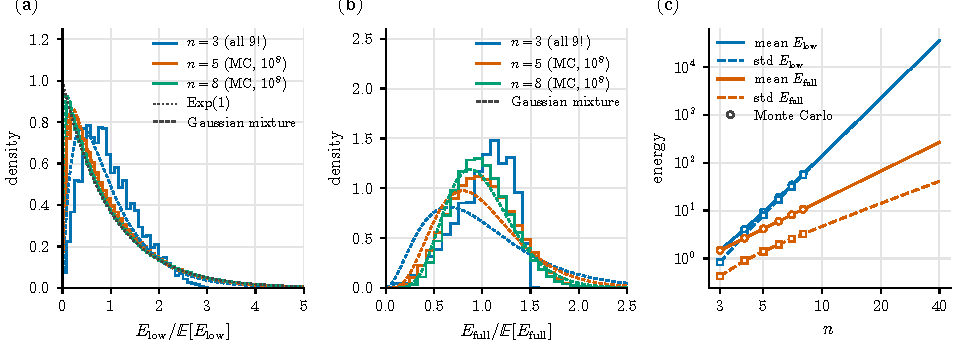
\includegraphics[width=0.92\textwidth]{figures/fig_random_energy.pdf}
\caption{Energy of a uniformly random arrangement. (a)~Distribution of $\Elow/\E[\Elow]$ for $n=3$ (all $9!$ arrangements) and $n=5,8$ ($10^8$ Monte Carlo samples each), with the densities of the Gaussian approximation (dashed) and the limit $\mathrm{Exp}(1)$ of \Cref{cor:random_energy_clt} (dotted). (b)~The same for $\Efull$, where the Gaussian approximation improves slowly (\Cref{rem:gauss_mixture}). (c)~Exact mean (solid) and standard deviation (dashed) of both energies for $3\le n\le40$, with Monte Carlo values for $3\le n\le8$ (open markers).}
\label{fig:random_energy}
\end{figure}
